% -*- Mode:TeX -*-
% LaTeX template for CinC papers                   v 1.1a 22 August 2010
%
% To use this template successfully, you must have downloaded and unpacked:
%       http://www.cinc.org/authors_kit/papers/latex.tar.gz
% or the same package in zip format:
%       http://www.cinc.org/authors_kit/papers/latex.zip
% See the README included in this package for instructions.
%
% If you have questions, comments or suggestions about this file, please
% send me a note!  George Moody (george@mit.edu)
%
\documentclass[twocolumn]{cinc}
\usepackage{graphicx}
\usepackage{amsmath}
\usepackage{amsfonts}

\begin{document}
\bibliographystyle{cinc}

\title{Multilabel 12-Lead Electrocardiogram Classification Using \\
Gradient Boosting Tree Ensemble}

\author {Alexander W. Wong$^{1}$, Weijie Sun$^{2}$, Sunil V. Kalmady$^{2}$, Padma Kaul$^{2}$, Abram Hindle$^{1}$\\
\ \\
 $^1$ University of Alberta, Edmonton, Canada \\
$^2$ Canadian VIGOUR Center, Edmonton, Canada }

\maketitle

\begin{abstract}

Standard 12-lead electrocardiograms (ECGs) are commonly used to detect cardiac irregularities such as atrial fibrillation, blocks, and irregular complexes.
For the PhysioNet/CinC 2020 Challenge, we built an algorithm using gradient boosted tree ensembles fitted on morphology and signal processing features.

For each lead, we derived features from heart rate variability, PQRST template shape, and full waveform duration.
We concatenated the features of all 12 leads to fit an ensemble of gradient boosting trees and predicted probabilities of ECG instances belonging to each class.
We used repeated random sub-sampling by splitting our dataset of 43,101 records into 100 independent runs of 85:15 training/evaluation splits for our evaluation results.

Our methodology generates an evaluation set challenge score of 0.484, with a PhysioNet official phase hold out test set score of 0.476 under the team name, CVC.

\end{abstract}

\section{Introduction}

The electrocardiogram (ECG) is the current "gold standard" strategy for detecting cardiac diseases, outperforming screening history and physical examinations in accuracy and sensitivity~\cite{harmon_effectiveness_2015}.
However, ECG interpretation is a complex task with frequent disagreements between health care staff, with up to a 33\% interpretation error rate~\cite{mele_improving_2008}.
Despite active research in computerized interpretations of ECGs, trained human over-reading and confirmation is required and emphasized in published reports~\cite{schlapfer_computer-interpreted_2017}.

This work classifies standard 12-lead ECGs to their clinical diagnosis as part of the \emph{PhysioNet/Computing in Cardiology Challenge}~\cite{physionet_challenge_2020}.
We developed a multi-label classification algorithm using entropy and signal processing inspired features and a gradient boosting tree ensemble.

\subsection{Dataset \& Scoring Criteria}

The official phase dataset contains a total of 43,101 ECG records.
Each record is labelled with a set of one or more SNOMED CT codes, although not all labels are evaluated in the challenge.
Table~\ref{tab:dataset_labeldx} displays the 27 labels selected for evaluation by the challenge organizers.

\begin{table}[htbp]
  \caption{\label{tab:dataset_labeldx} Labels count and percentage in dataset.}
  \vspace{4 mm}
  \centerline{\begin{tabular}{lrr} \hline
    Dx & Count & \% Total \\ \hline
    1st degree av block & 2394 & 5.6\% \\
    atrial fibrillation & 3475 & 8.0\% \\
    atrial flutter & 314 & 0.7\% \\
    bradycardia & 288 & 0.7\% \\
    complete right bundle branch block & 683 & 1.6\% \\
    incomplete right bundle branch block & 1611 & 3.7\% \\
    left anterior fascicular block & 1806 & 4.2\% \\
    left axis deviation & 6086 & 14.1\% \\
    left bundle branch block & 1041 & 2.4\% \\
    low qrs voltages & 556 & 1.3\% \\
    nonspecific intraventricular conduction & 997 & 2.3\% \\
    pacing rhythm & 299 & 0.7\% \\
    premature atrial contraction & 1729 & 4.0\% \\
    premature ventricular contractions & 188 & 0.4\% \\
    prolonged pr interval & 340 & 0.7\% \\
    prolonged qt interval & 1513 & 3.5\% \\
    q wave abnormal & 1013 & 2.4\% \\
    right axis deviation & 427 & 1.0\% \\
    right bundle branch block & 2402 & 5.6\% \\
    sinus arrhythmia & 1240 & 2.9\% \\
    sinus bradycardia & 2359 & 5.5\% \\
    sinus rhythm & 20846 & 48.4\% \\
    sinus tachycardia & 2402 & 5.6\% \\
    supraventricular premature beats & 215 & 0.5\% \\
    t wave abnormal & 4673 & 10.8\% \\
    t wave inversion & 1112 & 2.6\% \\
    ventricular premature beats & 365 & 0.8\% \\ \hline
  \end{tabular}}
\end{table}

The objective of this challenge is to maximize the metric: $\sum_{ij} w_{ij} a_{ij}$.
Given a set of diagnoses $C = \{c_i\}$, we compute a confusion matrix $A = [a_{ij}]$ where $a_{ij}$ contains records that are classified as class $c_i$ and belong to class $c_j$.
The weights $W = [w_{ij}]$, shown in Figure~\ref{fig:dataset_labeldx}, are set by the challenge to indicate clinical similarity between classes.


\begin{figure}[ht]
  \centering
  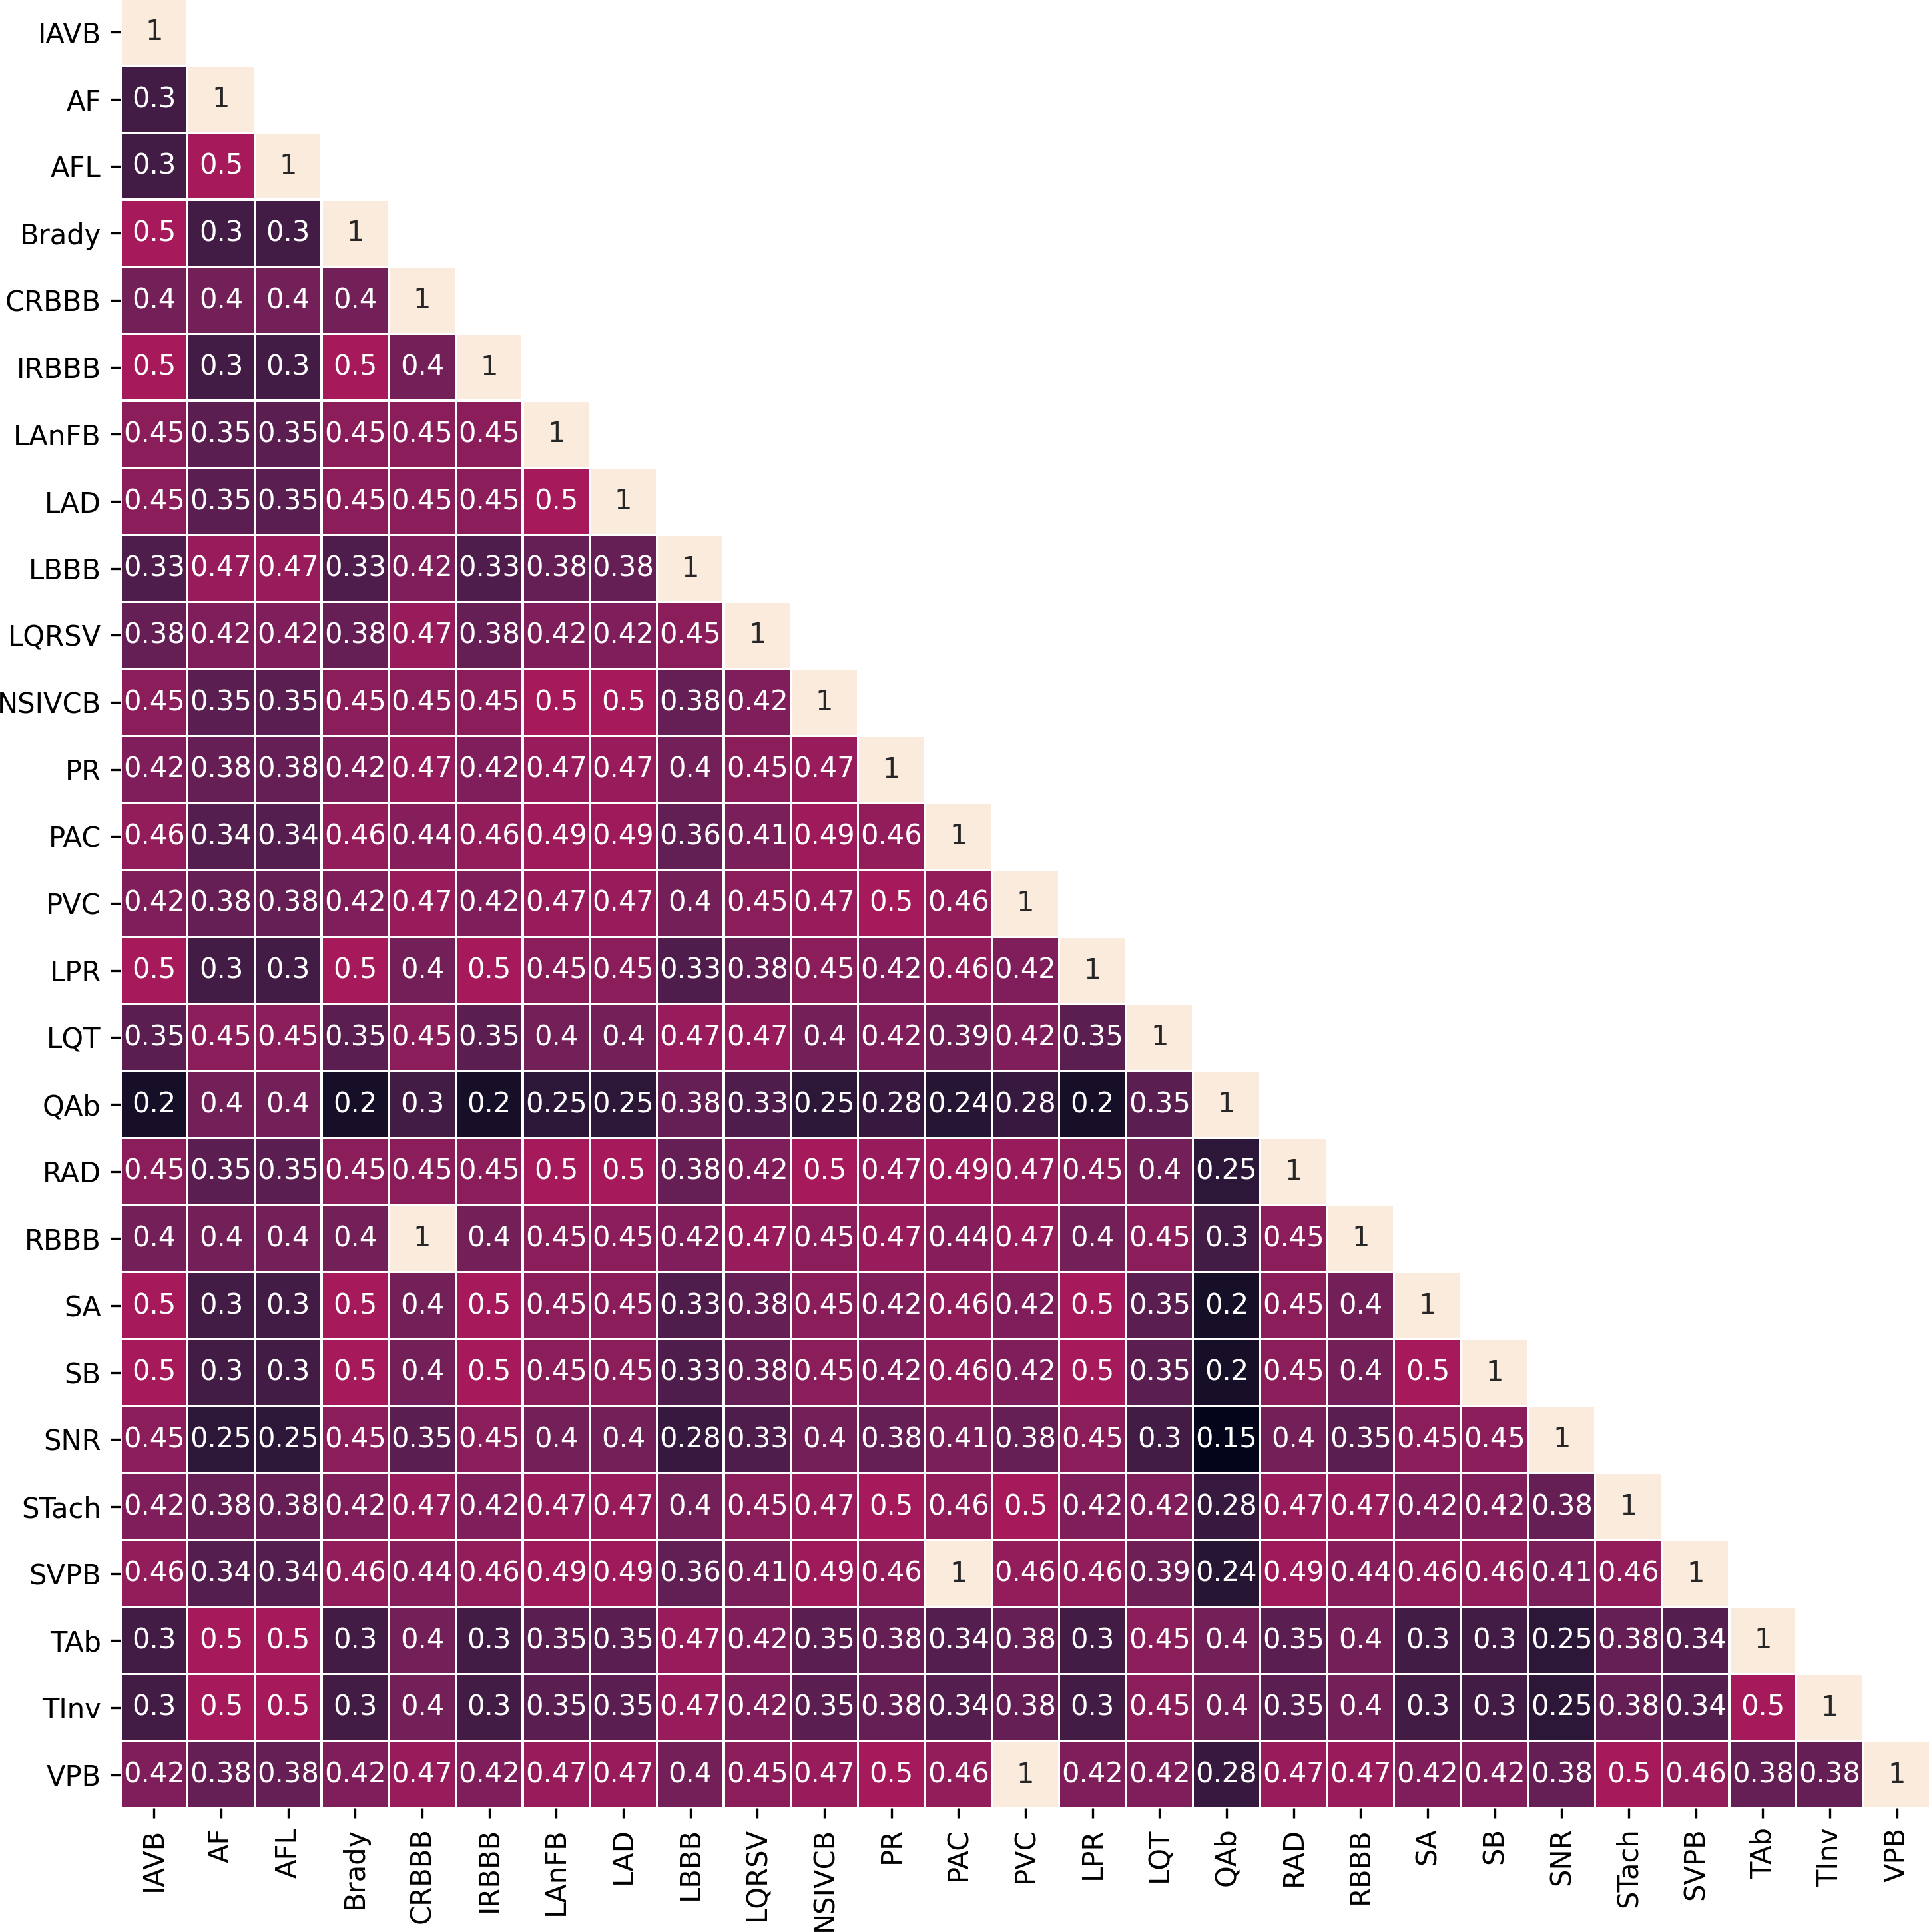
\includegraphics[width=8cm]{fig/label_weights.png}
  \caption{Evaluation scoring function weights per label.}
  \label{fig:dataset_labeldx}
\end{figure}

\section{Methodology}

Our approach is inspired by existing methods which use feature engineering and shallow learning classifiers~\cite{goodwin_classification_2017}.
An overview our methodology is presented in Figure~\ref{fig:methodology}.

Our feature extraction approach relies on the \emph{NeuroKit2} (version \texttt{0.0.40}) neurophysiological signal processing library for ECG signal cleaning, PQRST annotation, signal quality calculation, and heart rate variability metrics~\cite{neurokit2}.
Additionally, we use the general purpose time series feature extraction library \emph{tsfresh} (version \texttt{0.16.0}) for analysis of the PQRST template and the full waveform~\cite{CHRIST201872}.

\begin{figure}[ht]
  \centering
  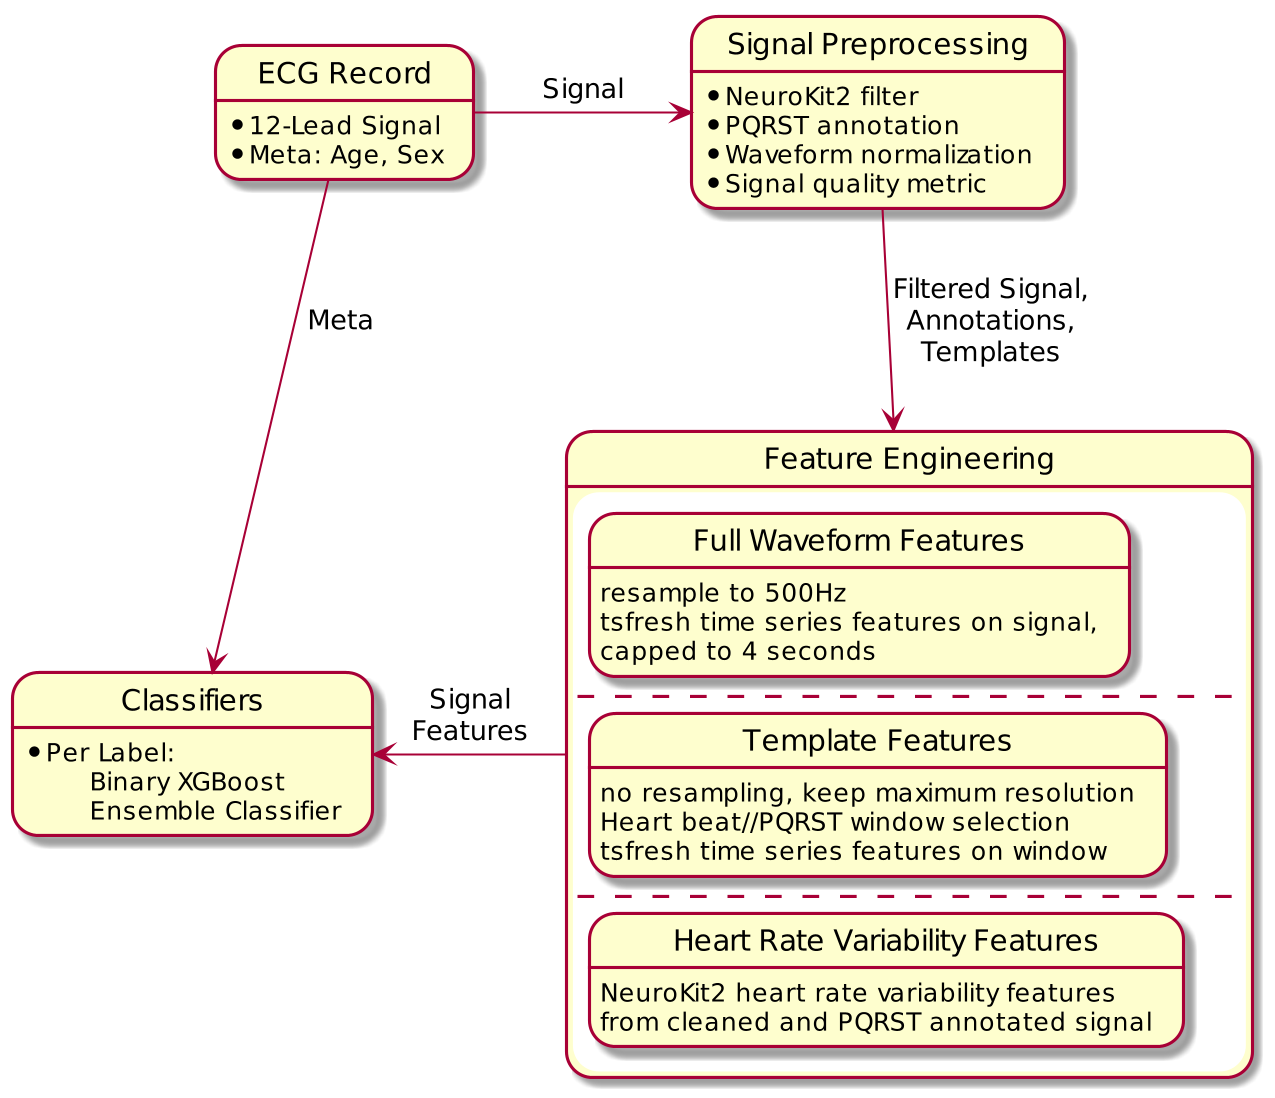
\includegraphics[width=7.9cm]{fig/methodology.png}
  \caption{Methodology overview. Feature engineering is performed concurrently for each lead then concatenated.}
  \label{fig:methodology}
\end{figure}

\subsection{Signal Pre-processing}

Prior to feature extraction and classification, we perform signal pre-processing to normalize and clean the raw ECG signal.
Slow drift and DC offset were removed with a Butterworth highpass filter followed by smoothing using a moving average kernel of size 0.02 seconds.
We treat each of the cleaned lead signals independently and annotated the PQRST peaks, the PRT onsets and offsets, and the atrial and ventricular systole and diastole phases.

We isolate one candidate heart beat signal for each lead by segmenting heart beat windows as a $-0.35$, 0.5 second window around each R-peak, shortening this window to $-0.25$ and 0.4 seconds if the mean heart rate exceeds 80 beats per minute.
We create an ECG signal quality metric by interpolating the distance of each QRS segment from the average QRS segment in the data.
ECG signal quality is therefore relative for each step in the entire length of the signal, where 1 corresponds to beats that are closest to the average QRS and 0 corresponds to beats that are most distant to the average QRS.
We chose the PQRST beat window with the highest signal quality as our candidate lead PQRST template.

\subsection{Feature Engineering}

Our engineered features can be categorized as one of three categories.
Full waveform features are derived using the end-to-end ECG signal.
Template features are constructed from the extracted PQRST window during pre-processing.
Heart rate variability features rely on the relative distances between each R-peak.
Each extraction technique was performed independently per lead.

For full waveform features, we used the cleaned ECG signal and applied the \emph{tsfresh} feature extraction library.
If the signal sampling rate exceeds 500Hz, we resampled down to 500Hz, otherwise the maximum sampling rate resolution was used.
We further limited the signal to the middle 2000 samples, or 4 seconds at 500Hz, to remove starting and trailing artifacts.
We set the \texttt{ComprehensiveFCParameters} parameter during \emph{tsfresh} feature extraction.
From each lead, we generated 763 full waveform features.

Template features were derived from the isolated heart beat window with highest signal quality.
No downsampling or truncation was performed due to the short duration of the extracted templates.
The \emph{tsfresh} feature extraction settings remained unchanged from the full waveform features.
We generated 763 template features per lead.

Heart rate variability (HRV) features reported by \emph{NeuroKit2} were calculated using the cleaned signal and corresponding signal annotations.
The relative R-peak distances were the primary inputs for these generated features.
For each lead, 53 different HRV features were generated.

For each 12-lead record we combined all three categories of engineered features with the age and sex parsed from the ECG record metadata.
We arrived at a $12 * (763 + 763 + 53) + 2 = 18,950$ length feature vector per 12-lead record.
For undefined features, such as the HRV feature set on signals where no PQRST annotations could be generated, \texttt{NaN} placeholders were set.

\subsection{Classification}

We trained a XGBoost binary classifier for each of the 27 clinical diagnosis, using \texttt{xgboost@1.1.1}~\cite{chen_xgboost_2016}.
We used the \texttt{gbtree} booster method with the \texttt{gpu\_hist} tree method and \texttt{gradient\_based} sampling method.
All other model parameters were left to their defaults.

The evaluation scoring function weights were used during training as instance sample weights, capping positive examples to a 0.5 threshold.
For example, when training the 1st degree av block (IAVB) classifier we also considered instances of bradycardia (Brady), incomplete right bundle branch block (IRBBB), prolonged PR interval (LPR), sinus arrhythmia (SA), and sinus bradycardia (SB) as positive examples with 0.5 weight.
Other labels that had scoring function weights below 0.5 were treated as negative examples with a sample weight of 1.
To account for the dataset label imbalance, we further scaled the positive example weight using the number of negative examples over the positive examples in the training set split.
We used repeated random sub-sampling of our total dataset, randomly splitting our 43,101 records into an 85:15 training/evaluation set split.

We ran 100 experiments using the full 18,804 features to determine the feature importances.
We calculated the average feature importance for each feature from all the experiments and models for each of the labels.
Our challenge classification results were generated from training 100 additional models using only the top 1,000 most important features, ranked by mean feature importance.

\section{Results}

\begin{figure}[ht]
  \centering
  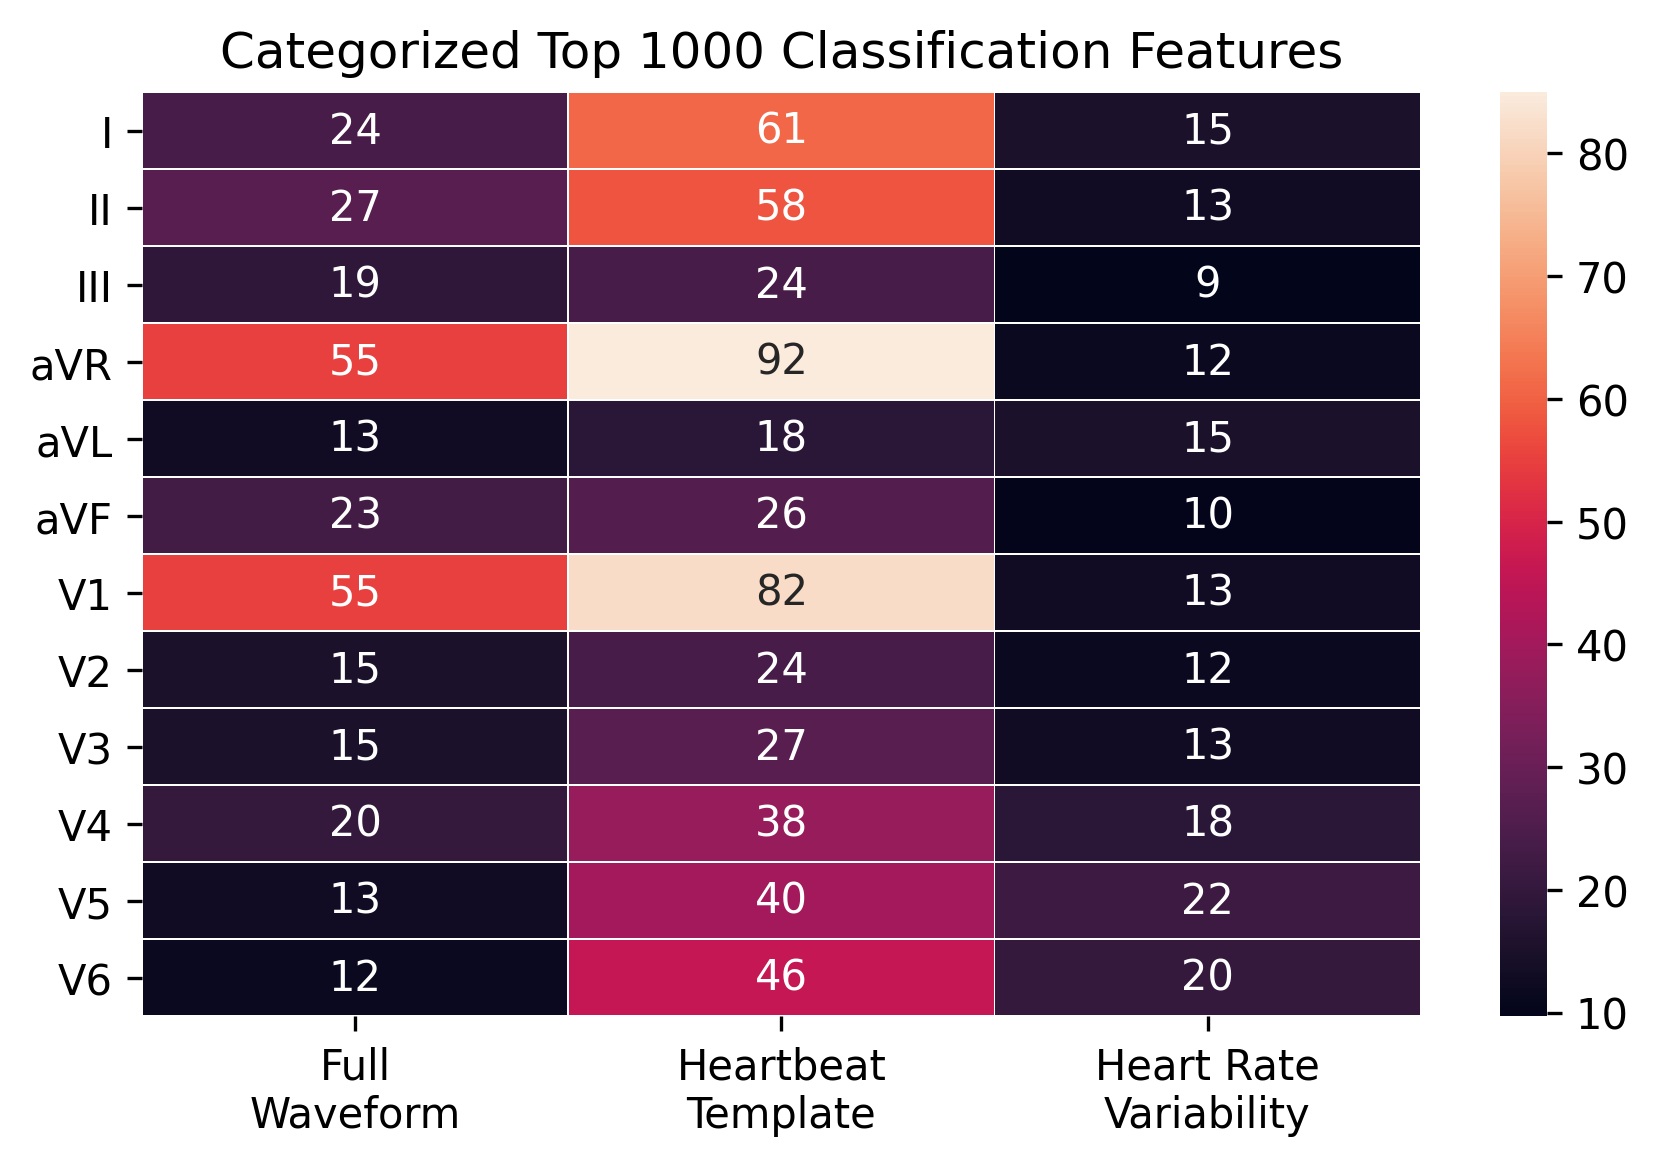
\includegraphics[width=7.9cm]{fig/top_features.png}
  \caption{Breakdown of the top 1,000 XGBoost features. Age is an important feature, while sex is not important.}
  \label{fig:top_features}
\end{figure}

A categorical visualization of our top 1000 features, broken down by lead and feature type, is shown in Figure~\ref{fig:top_features}.
Our methodology attained a mean challenge metric score of 0.484 on our evaluation set.
Additionally, we attained mean values for AUROC of 0.890, AUPRC of 0.390, accuracy of 0.251, overall $\text{F}_1$ score of 0.370, $\text{F}_\beta$ of 0.427, and $\text{G}_\beta$ measure of 0.222.
The challenge provided scoring code defined $\beta = 2$.
An overview of the experiment classification metrics can be found in Figure~\ref{fig:classification_metrics_summary}.

\begin{figure}[hb]
  \centering
  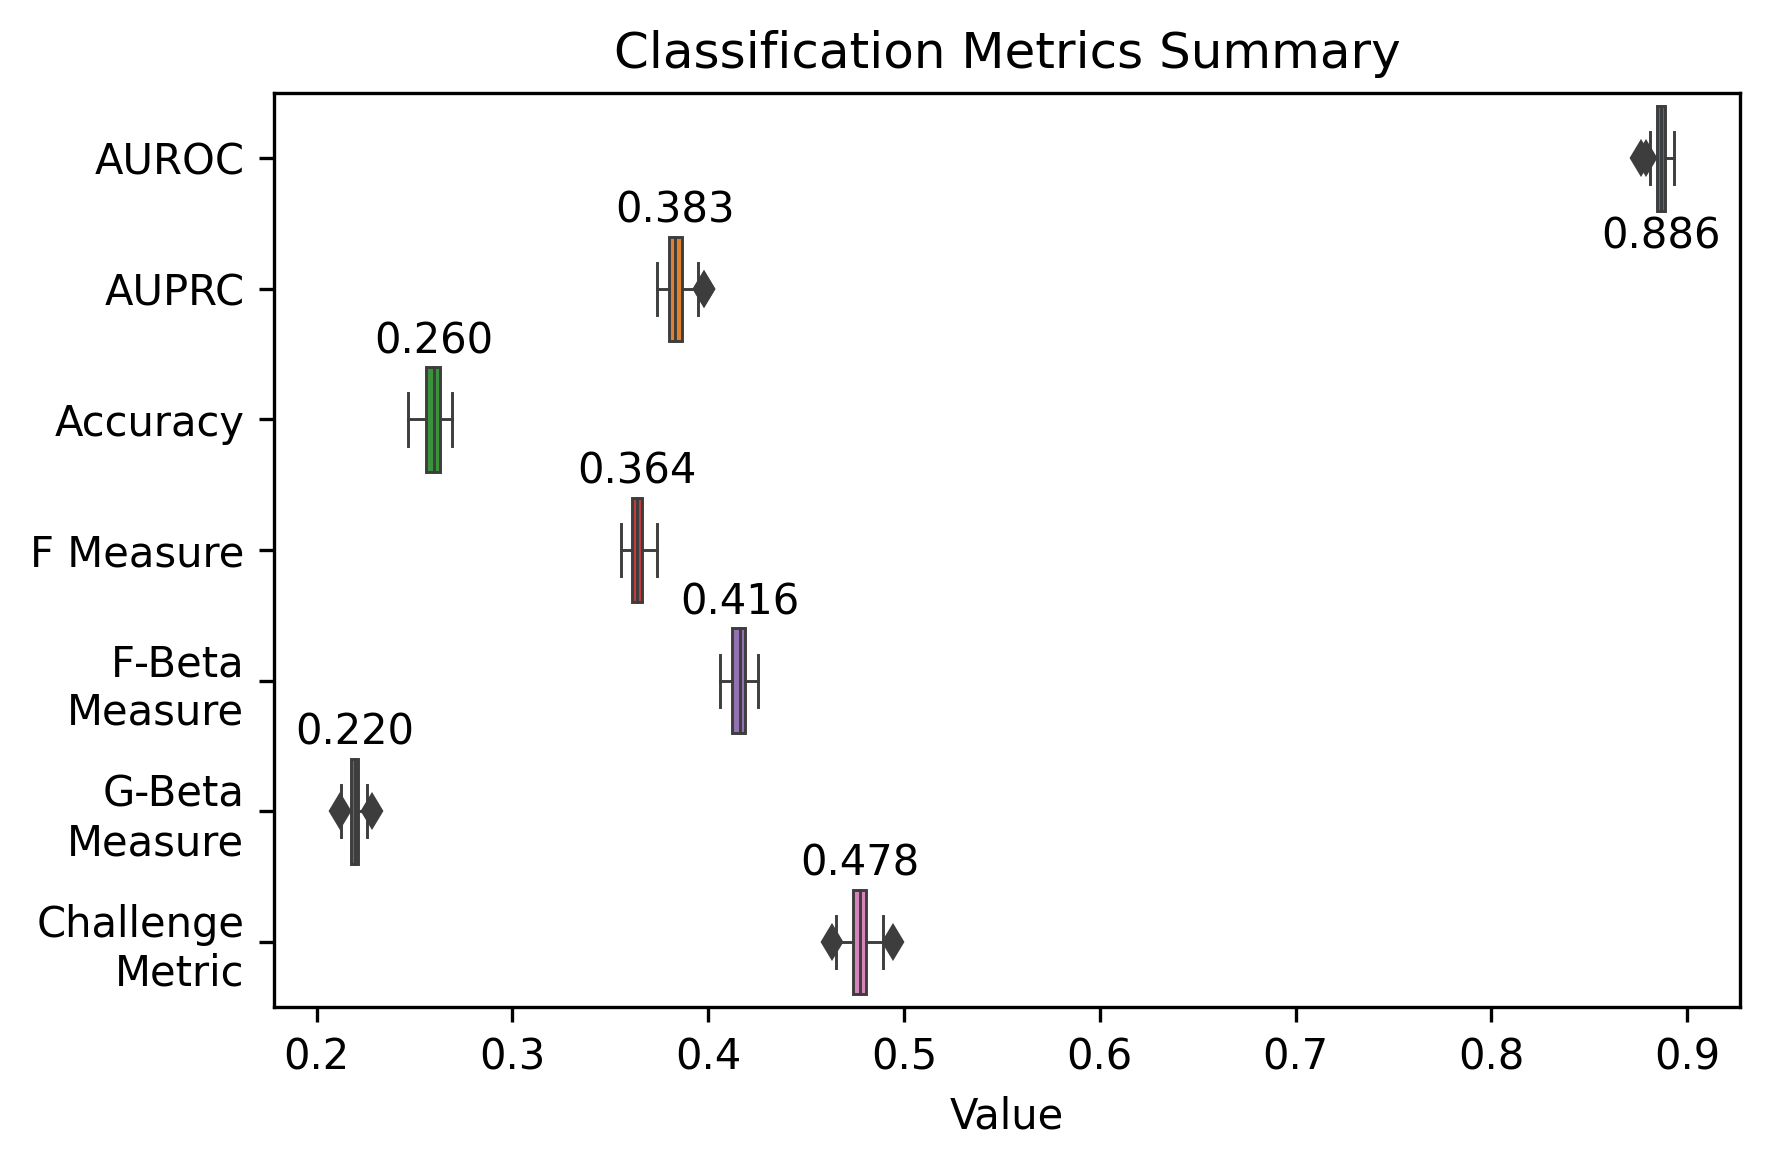
\includegraphics[width=7.9cm]{fig/classification_metrics.png}
  \caption{Summary of classification metrics over 100 experiments on all labels. Annotations indicate mean value.}
  \label{fig:classification_metrics_summary}
\end{figure}

Our model's top three best classified labels are normal sinus rhythm (SNR, $\text{F}_1$ mean: 0.920), right bundle branch block (RBBB, $\text{F}_1$ mean: 0.853), and left bundle branch block (LBBB, $\text{F}_1$ mean: 0.836).
The summary of our 100 experiment $\text{F}_1$ scores for each label is in Figure~\ref{fig:f1_score}.

\begin{figure*}[ht]
  \centering
  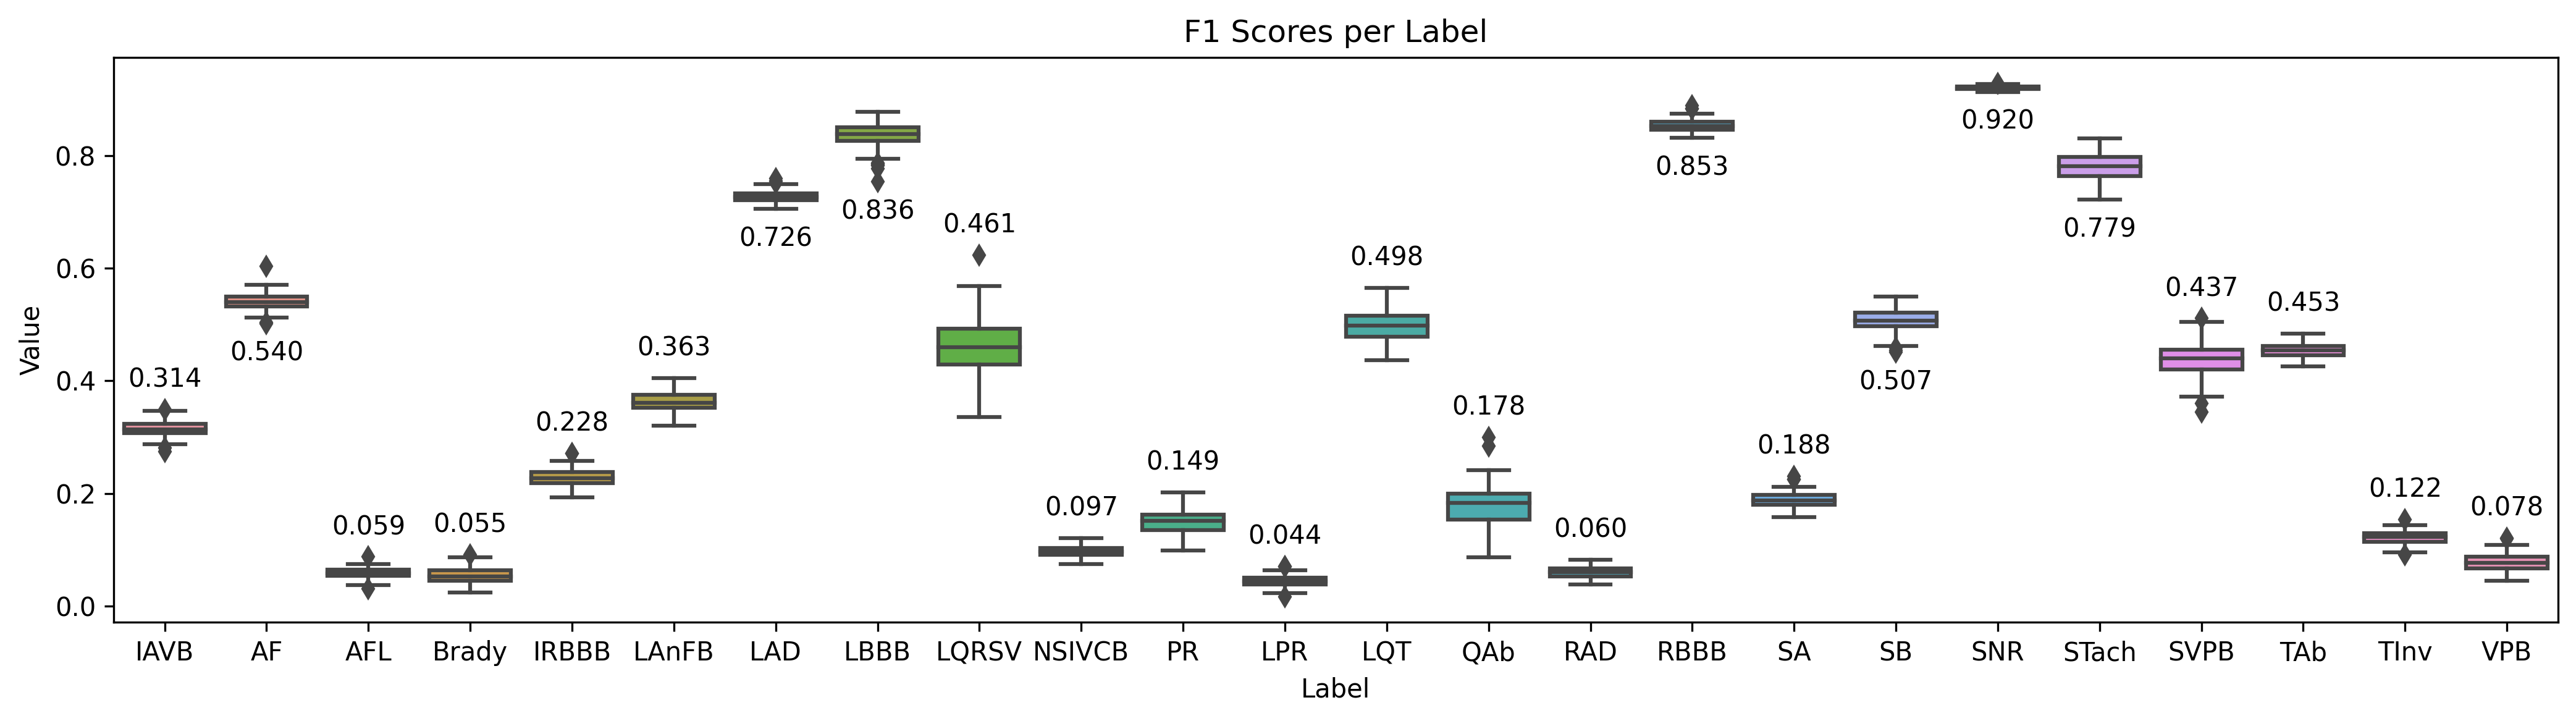
\includegraphics[width=17.0cm]{fig/label_f1s.png}
  \caption{Label-wise $\text{F}_1$ scores over 100 experiments. Annotations indicate mean value.}
  \label{fig:f1_score}
\end{figure*}

Furthermore, we ran a Pearson correlation coefficient test between the label $\text{F}_1$ means and the label counts within our dataset.
The statistical test revealed a Pearson correlation coefficient of 0.568 at a p-value of $3.8 \cdot 10^{-3}$.
This result suggests that a positive linear correlation exists between the label occurrence in our dataset and our classification model's $\text{F}_1$ score.
On the official phase hold out test set, our methodology achieved a challenge score of 0.476.


\section{Discussion \& Future Work}

Despite the label specific scaling of our dataset training weights, the correlation between the label occurrence with the $\text{F}_1$ scores revealed further improvements are necessary to address the existing label imbalance.
The label imbalance may be addressed by adding more low occurrence disorders into the existing corpus of ECG records.
Synthesizing new records of low occurrence disorders to use as training data may also prove promising.
Additionally, exploration of new features to use as classifier inputs may reveal common characteristics of specific heart disorders that are currently unused or missing.

Our approach, although applicable to 12-lead ECGs, perform feature extraction on each lead separately before concatenating the features together for classification.
We believe that further improvements can be made utilizing feature extraction approaches capable of handling multi-dimensional time series data.

\section{Conclusion}

We created an algorithm for the classification of 27 heart conditions using natural language and signal processing inspired feature engineering and an XGBoost tree ensemble classifier.
We combined a set of 18,804 features from full waveform, template, and heart rate variability groups.
Using 100 repeated random sub-sampling of 85:15 train/evaluation, we trained models to get feature importances and distilled out 1,000 most important features.
Using this reduced set of 1,000 features, we retrained our models and achieved a mean challenge score of 0.484 on our evaluation split.
The official phase challenge score on PhysioNet's hold out test set is 0.476 for our team, \emph{CVC}.


\section*{Acknowledgments}
We would like to thank Eric Ly and Leiah Luoma of the Canadian VIGOUR Center for their help and guidance during our research journey.

\bibliography{main}

\begin{correspondence}
Alexander W. Wong\\
Department of Computing Science\\
2-32 Athabasca Hall, University of Alberta\\
Edmonton, Alberta, Canada\\
T6G 2E8\\
alex.wong@ualberta.ca
\end{correspondence}

\end{document}

